% Copyright (c) 2005 Nokia Corporation
%
% Licensed under the Apache License, Version 2.0 (the "License");
% you may not use this file except in compliance with the License.
% You may obtain a copy of the License at
%
%     http://www.apache.org/licenses/LICENSE-2.0
%
% Unless required by applicable law or agreed to in writing, software
% distributed under the License is distributed on an "AS IS" BASIS,
% WITHOUT WARRANTIES OR CONDITIONS OF ANY KIND, either express or implied.
% See the License for the specific language governing permissions and
% limitations under the License.

\section{\module{calendar} ---
  Access to calendar related services}
\label{sec:calendar}

\declaremodule{extension}{calendar}
\platform{S60}
\modulesynopsis{A calendar related services package.}

The \module{calendar} module offers an API to calendar services. The 
\module{calendar} module represents a Symbian agenda database as a 
dictionary-like \class{CalendarDb} object, which contains \class{Entry}
objects and which is indexed using the unique IDs of those objects. There 
are four types of entry objects: \class{AppointmentEntry}, 
\class{EventEntry}, \class{AnniversaryEntry}, and \class{TodoEntry}. 

\class{CalendarDb} objects represent a live view into the database. If an 
entry is changed outside your Python application, the changes are visible 
immediately, and conversely any changes you commit into the database are 
visible immediately to other applications. 

In addition to entries, there are todo lists which contain todo entries. 
Todo lists are accessed using the dictionary-like \class{TodoListDict} and 
\class{TodoList} objects.

All time parameters use Unix time unless stated otherwise. For more 
information on Unix time, see Section \ref{subsec:datetime}, 
Date and Time.

\begin{figure}
\centering
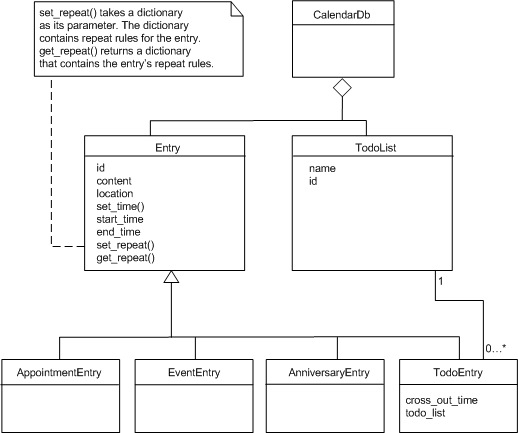
\includegraphics[width=10cm]{libcalendar-1}
\caption{The \module{calendar} module objects}
\label{libcalendar-1}
\end{figure}

Figure \ref{libcalendar-1} demonstrates the relationships of the 
\code{calendar} module objects. 

\subsection{Module Level Functions}
\label{subsec:calendarmodule}
The following free functions - functions that do not belong to any class 
- are defined in the \code{calendar} module:

\begin{funcdesc}{open}{\optional{filename=None, mode=None}}

Opens a calendar database and returns a new \class{CalendarDb} object.

If filename is \code{None}, the default database is opened.

If \var{filename} is given, it should be a full, absolute path name in
Unicode that specifies the calendar database to open. 

\var{mode} can be:

\begin{itemize}
\item \code{None}: Opens an existing calendar database.
\item \code{'c'}: Opens an existing calendar database, or creates it if it doesn't exist.
\item \code{'n'}: Creates a new, empty calendar database. If \var{filename} exists, the previous contents are erased.
\end{itemize}

\end{funcdesc}

\subsection{CalendarDb Objects}
\label{subsec:calendardb}

Calendar entries and todo lists are stored in a calendar database. There is 
one default calendar database but more calendar databases can be created by 
invoking \code{open} with parameters \code{'n' }or \code{'c'}. 

\begin{classdesc*}{CalendarDb}
\class{CalendarDb} objects have the following methods:

\begin{methoddesc}[CalendarDb]{add_appointment}{}

Creates and returns a new appointment entry \class{AppointmentEntry}. The 
entry is not added and saved into the database until \code{Entry.commit} is 
called.

\end{methoddesc}

\begin{methoddesc}[CalendarDb]{add_event}{}

Creates and returns a new event entry \class{EventEntry}. The entry is not added 
and saved into the database until \code{Entry.commit} is called.

\end{methoddesc}

\begin{methoddesc}[CalendarDb]{add_anniversary}{}

Creates and returns a new anniversary entry \class{AnniversaryEntry}. The entry 
is not added and saved into the database until \code{Entry.commit} is called.

\end{methoddesc}

\begin{methoddesc}[CalendarDb]{add_todo}{}

Creates and returns new todo entry \class{TodoEntry}. The entry is not added and 
saved into the database until \code{Entry.commit} is called.

\end{methoddesc}

\begin{methoddesc}[CalendarDb]{find_instances}{start_date, end_date, search_str=u''\optional{ ,appointments=0,events=0,anniversaries=0,todos=0}}

The parameters for this function include the start date, end date, search 
string, and optional parameters. The optional parameters define the entry 
types to be included into the search. By default all entry types are 
included. Returns a list that contains \class{Entry} instances found in the 
search. An instance is a dictionary that contains the entry ID and the 
datetime value. An entry may have several instances if it is repeated, for 
example once every week, etc. However, all the returned instances occur on 
the same day, i.e. on the first day between the start and end datetime 
values that contains instances. To search all instances between the initial 
start and end datetime values, you may have to execute several searches and 
change the start datetime value for each search. A match is detected if the 
search string is a substring of an entry's content. 

\end{methoddesc}

\begin{methoddesc}[CalendarDb]{monthly_instances}{month, appointments=0, events=0, anniversaries=0, todos=0}

The parameters for this function include \var{month} (float) and 
optional parameters. The optional parameters define the entry types to be 
returned. Returns a list that contains entry instances occurring during the 
specified calendar month.

\end{methoddesc}

\begin{methoddesc}[CalendarDb]{daily_instances}{day, appointments=0, events=0, anniversaries=0, todos=0}

The parameters for this function include \var{day} (float) and 
optional parameters. The optional parameters define the entry types to be 
returned. Returns a list that contains entry instances occurring on the 
specified day.

\end{methoddesc}

\begin{methoddesc}[CalendarDb]{add_todo_list}{\optional{name=None}}

Creates a new todo list. \var{name} sets the name of the todo list 
(Unicode). Returns the ID of the created todo list.

\end{methoddesc}

\begin{methoddesc}[CalendarDb]{export_vcalendars}{(int,...)}

Returns a \code{vcalendar} string that contains the specified entries in 
vCalendar format. The parameter for this function is a tuple that contains 
the entry IDs of the exported entries.

\end{methoddesc}

\begin{methoddesc}[CalendarDb]{import_vcalendars}{string}

Imports \code{vcalendar} entries, given in the string parameter, to the 
database. Returns a tuple that contains the unique IDs of the imported 
entries.

\end{methoddesc}

\begin{memberdesc}[CalendarDb]{todo_lists}

Contains a dictionary-like \code{TodoListDict} object for accessing
the todo lists of this database.

\end{memberdesc}

\begin{methoddesc}[CalendarDb]{__delitem__}{id}

Deletes the given calendar \code{Entry} from the database. \code{id} is the 
unique ID of the calendar \code{Entry}.

\end{methoddesc}

\begin{methoddesc}[CalendarDb]{__getitem__}{id}

Returns a calendar \code{Entry} object indicated by the unique ID. The returned 
object can be one of the following: \class{AppointmentEntry}, 
\class{EventEntry}, \class{AnniversaryEntry}, or \class{TodoEntry}. \code{id} is 
the unique ID of the calendar \code{Entry}. 

\end{methoddesc}

\begin{methoddesc}[CalendarDb]{compact}{}

Compacts the database file. The returned value (integer) indicates the 
success of compaction; a value other than zero means that the compaction was 
successful.

\end{methoddesc}

\end{classdesc*}

\subsection{Entry Objects}
\label{subsec:entry}

An \class{Entry} object represents a live view into the state of a single 
entry in the database. You can access the entries with an entry's unique ID. 
If you create a new entry using \code{db.add_appointment} etc., it is 
saved into the database only if you call the entry's \code{commit} method. 
In case an entry is already saved into the database, the autocommit mode is 
on by default and all the changes are automatically saved into the database, 
unless you call the entry's \code{begin} method. If you call the entry's 
\code{begin} method, the changes are not saved into the database until you 
call the entry's \code{commit} method. 

Database entries cannot be locked. In other words, other applications are 
able to make changes to the database entries you are using (not directly to 
the \class{EntryObjects} you are using, but to their representation in the 
database) at the same time you are modifying them, even if you use 
\code{begin} and \code{commit} methods. 

\begin{classdesc*}{Entry}
\class{Entry} objects have the following methods and properties:

\begin{memberdesc}[Entry]{content}

Sets or returns the entry's content text (Unicode).

\end{memberdesc}

\begin{methoddesc}[Entry]{commit}{}

Saves the entry or in case of a new entry adds the entry into the database. 
Note that this can be called only in case of a new entry, created with 
\code{db.add_appointment} etc., or after \code{begin} is called. 

\end{methoddesc}

\begin{methoddesc}[Entry]{rollback}{}

Undoes the changes made after last \code{commit}.

\end{methoddesc}

\begin{methoddesc}[Entry]{set_repeat}{dictionary}

Sets the repeat data of the entry. \var{dictionary} is a repeat data dictionary 
that contains all the repeat rules. For more information on repeat rules, see 
Section \ref{subsec:repeat}, Repeat Rules.

\end{methoddesc}

\begin{methoddesc}[Entry]{get_repeat}{}

Returns the repeat data dictionary of the entry.

\end{methoddesc}

\begin{memberdesc}[Entry]{location}

Sets or returns the entry's location data (Unicode), for example meeting 
room information. 

\end{memberdesc}

\begin{methoddesc}[Entry]{set_time}{start\optional{, end}}

Sets the start and end datetime values of the entry (floats). If only one 
parameter is given, the other will have the same value. 

In case of events, anniversaries, and todo entries the datetime values are 
truncated to corresponding date values.

\class{TodoEntries} can be made undated with 
\code{TodoEntry.set_time(None)}. Making the todo entry undated means 
removing the start and end date and all the repeat rules.

\end{methoddesc}

\begin{memberdesc}[Entry]{start_time}

The start datetime value (float) of the entry or \code{None} if 
the start datetime of the entry is not set.

\end{memberdesc}

\begin{memberdesc}[Entry]{end_time}

The end datetime value (float) of the entry or \code{None} if the 
end datetime of the entry is not set.

\end{memberdesc}

\begin{memberdesc}[Entry]{id}

The unique ID of the entry.

\end{memberdesc}

\begin{memberdesc}[Entry]{last_modified}

The datetime value (float) of the entry's last modification in 
universal time.

\end{memberdesc}

\begin{memberdesc}[Entry]{alarm}

The alarm datetime value (float) for the entry. \code{None} if \code{alarm} is 
not set. Alternatively removes the alarm if the value is set to \code{None}. 

Alarms can be set to all \class{Entry} types. However, only alarms set to 
Appointments and Anniversaries will actually cause an alarm; this is similar 
to the Calendar application in your Nokia device, which allows you to set an 
alarm only for Meetings and Anniversaries. In addition, alarms set to any 
entries residing in a database other than the default database do not cause 
actual alarms either.

\end{memberdesc}

\begin{memberdesc}[Entry]{priority}

The priority of the entry, which can be an integer ranging from 0 to 255. Native 
Phonebook and Calendar applications in Nokia devices use value 1 for high 
priority, 2 for normal priority, and 3 for low priority. 

\end{memberdesc}

\begin{memberdesc}[Entry]{crossed_out}

The crossed out value of an entry. A value that is interpreted as false means 
that the entry is not crossed out, whereas a value that is interpreted as true 
means that the entry is crossed out. Note that \class{TodoEntries} must also 
have a cross-out time while the other entry types cannot have one. If 
\class{TodoEntry} is crossed out using this method, the moment of crossing out 
is set to the cross-out time of the \class{TodoEntry}. See also Section 
\ref{subsubsec:todoentry}, TodoEntry, \code{cross_out_time}.

\end{memberdesc}

\begin{memberdesc}[Entry]{replication}

Sets or returns the entry's replication status, which can be one of the 
following: \code{'open'}, \code{'private',} or \code{'restricted'}.

\end{memberdesc}

\begin{methoddesc}[Entry]{as_vcalendar}{}

Returns this entry as a vCalendar string.

\end{methoddesc}

\end{classdesc*}

\subsubsection{AppointmentEntry Objects}
\label{subsubsec:appointmententry}

\begin{classdesc*}{AppointmentEntry}
\end{classdesc*}

\class{AppointmentEntry} class contains no additional methods compared to 
the \class{Entry} class from which it is derived.

\subsubsection{EventEntry}
\label{subsubsec:evententry}

\begin{classdesc*}{EventEntry}
\end{classdesc*}

\class{EventEntry} class contains no additional methods compared to the 
\class{Entry} class from which it is derived.

\subsubsection{AnniversaryEntry}
\label{subsubsec:anniversaryentry}

\begin{classdesc*}{AnniversaryEntry}
\end{classdesc*}

\class{AnniversaryEntry} class contains no additional methods compared to 
the \class{Entry} class from which it is derived.

\subsubsection{TodoEntry}
\label{subsubsec:todoentry}

\class{TodoEntry}objects represent todo entry types. They have additional 
properties compared to the \class{Entry} class from which they are derived.

\begin{classdesc*}{TodoEntry}
\class{TodoEntry}objects have the following additional properties:

\begin{memberdesc}[TodoEntry]{cross_out_time}

The cross-out date value of the entry. The value can be \code{None} meaning that 
the entry is not crossed out, or the cross-out date (float). The set value must 
be date (float). Setting a cross-out time also crosses out the entry. See also 
Section \ref{subsec:entry}, Entry Object, \code{crossed_out}.

\end{memberdesc}

\begin{memberdesc}[TodoEntry]{todo_list}

The ID of the todo list to which this entry belongs.

\end{memberdesc}

\end{classdesc*}

\subsubsection{TodoListDict}
\label{subsubsec:todolistdict}

\class{TodoListDict} objects are dictionary-like objects that enable 
accessing todo lists. 

\begin{classdesc*}{TodoListDict}
\class{TodoListDict} objects have the following property:

\begin{memberdesc}[TodoListDict]{default_list}

The ID of the default todo list.

\end{memberdesc}

\end{classdesc*}

\subsubsection{TodoList}
\label{subsubsec:todolist}

\class{TodoList} objects are dictionary-like objects that enable 
accessesing todo lists. 

\begin{classdesc*}{TodoList}
\code{TodoList} objects have the following properties:

\begin{memberdesc}[TodoList]{name}

The name of the todo list as a Unicode string.

\end{memberdesc}

\begin{memberdesc}[TodoList]{id}

Returns the ID of the todo list as an integer.

\end{memberdesc}

\end{classdesc*}

\subsection{Repeat Rules}
\label{subsec:repeat}

Repeat rules specify an entry's repeat status, that is, the recurrence of 
the entry. There are six repeat types: 

\begin{itemize}
\item \code{daily}: repeated daily
\item \code{weekly}: repeat on the specified days of the week, such as Monday and Wednesday, etc.
\item \code{monthly_by_dates}: repeat monthly on the specified dates, such as the 15th and 17th day of the month
\item \code{monthly_by_days}: repeat monthly on the specified days, such as the fourth Wednesday of the month, or the last Monday of the month
\item \code{yearly_by_date}: repeat yearly on the specified date, such as December 24
\item \code{yearly_by_day}: repeat yearly on the specified day, such as every third Tuesday of May
\end{itemize}

There are exceptions to repeat rules. For example, you can specify the 
datetime value (float) in such a way that the entry is not repeated on a 
specific day even if the repeat rule would specify otherwise.

You must set the start and end dates (floats) of the repeat. The end date 
can also be set to \code{None} to indicate that the repeating continues 
forever. You can set \code{interval} defining how often the repeat occurs, 
for example in a daily repeat: \code{1} means every day, \code{2} means 
every second day, etc. You can also set the \code{days} specifier which 
lets you explicitly specify the repeat days; for example in a weekly repeat 
you can set \code{"days":[0,2]} which sets the repeat to occur on Mondays 
and Wednesdays. If you do not set the \code{days} specifier, the repeat 
days are calculated automatically based on the start date.

You can modify repeat data by calling \code{rep_data = 
entry.get_repeat()}, then making changes to \code{rep_data} 
dictionary, and then calling \code{entry.set_repeat(rep_data)}.

Repeating can be cancelled by calling \code{entry.set_repeat} with a 
parameter that is interpreted to be false, such as 
\code{entry.set_repeat(None)}.

Repeat definition examples:

\begin{verbatim}

repeat = {"type":"daily", #repeat type
          "exceptions":[exception_day, exception_day+2*24*60*60],  
          #no appointment on those days
          "start":appt_start_date, #start of the repeat
          "end":appt_start_date+30*24*60*60, #end of the repeat
          "interval":1} #interval (1=every day, 2=every second day etc.)

repeat = {"type":"weekly", #repeat type
          "days":[0,1], #which days in a week (Monday, Tuesday)
          "exceptions":[exception_day], #no appointment on that day
          "start":appt_start_date, #start of the repeat
          "end":appt_start_date+30*24*60*60, #end of the repeat
          "interval":1}  
          #interval (1=every week, 2=every second week etc.) 

repeat = {"type":"monthly_by_days", #repeat type
          # appointments on second Tuesday and last Monday of the month
          "days":[{"week":1, "day":1},{"week":4, "day":0}],
          "exceptions":[exception_day], #no appointment on that day 
          "start":appt_start_date, #start of the repeat
          "end":appt_start_date+30*24*60*60, #end of the repeat
          "interval":1}  
          #interval (1=every month, 2=every second month etc.)

repeat = {"type":"monthly_by_dates", #repeat type
          "days":[0,15],  
          # appointments on the 1st and 16th day of the month.
          "exceptions":[exception_day], #no appointment on that day
          "start":appt_start_date, #start of the repeat
          "end":appt_start_date+30*24*60*60, #end of the repeat
          "interval":1}  
          #interval (1=every month, 2=every second month etc.)

repeat = {"type":"yearly_by_date", #repeat type
          "exceptions":[exception_day], #no appointment on that day 
          "start":appt_start_date, #start of the repeat
          "end":appt_start_date+3*365*24*60*60, #end of the repeat
          "interval":1}  
          #interval (1=every year, 2=every second year etc.)

repeat = {"type":"yearly_by_day", #repeat type
          # appointments on the second Tuesday of February
          "days":{"day":1, "week":1, "month":1},
          "exceptions":[exception_day], #no appointment on that day 
          "start":appt_start_date, #start of the repeat
          "end":appt_start_date+3*365*24*60*60, #end of the repeat
          "interval":1}  
          #interval (1=every year, 2=every second year etc.)

\end{verbatim}
